\documentclass[11pt]{ltjsarticle}

\usepackage{fontspec}
%\setmainfont[BoldFont=Times Bold, ItalicFont=Times Italic, BoldItalicFont=Times Bold Italic]{Times}
%\setsansfont[BoldFont=Helvetica Neue Bold, ItalicFont=Helvetica Neue Italic, BoldItalicFont=Helvetica Neue Bold Italic]{Helvetica Neue}
%\setmonofont{Menlo}
\usepackage{luatexja-fontspec}
\usepackage[hiragino-pron]{luatexja-preset}
\usepackage{luatexja-ruby}
\usepackage{graphicx}



%\renewcommand{\headfont}{\bfseries\sffamily

\title{電気電子計算工学及演習}
\author{三軒家 佑將(さんげんや ゆうすけ) \\ 3回生 \\ 1026-26-5817 \\ a0146089}
\date{}

\begin{document}
\maketitle


以下のレポートにおいては、プログラミング言語としてGo言語(https://goo.gl/pclkeC)を用いた。

また、ソースコードは巻末にまとめて添付した。

\section{採用したアルゴリズム}
\subsection{行列とベクトルの演算を行う関数の実装}
	行列ベクトル積の演算を行う関数MatVecと、行列積の演算を行う関数MatMltを、ソースコード1のとおりに実装した。
	\subsubsection*{MatVec}
		行列ベクトル積の演算は、「引数の行列の各行ベクトル」と、引数のベクトルの内積を並べたものと考えることができる。
		この考えに則り、ベクトルの内積を計算する補助関数dotを定義し、それを用いて行列ベクトルの計算を行った。
	\subsubsection*{MatMlt}
		行列積の演算は、引数1の行列と「引数2の行列の各列ベクトル」の行列ベクトル積を並べたものと考えることができる。
		この考えに則り、MatVec関数を用いて行列積の計算を行った。

\subsection{バッタGの移動}
	ある時刻tの存在確率ベクトル(地点0,1,2,3,4,5にいる確率を並べたもの)${\bf p}_t$は、
	\[
		{\bf p}_t = {\bf A}{\bf p}_{t-1}
	\]
	によって求めることができる。ただし{\bf A}は、表1の数値部分を行列と考え、さらにそれの転置を取ったものである。
	
	この考え方に則って、バッタGが、ある時刻$0 \leq t \leq 60$に地点0,1,2,3,4,5にいる確率を計算した(ソースコード2)。

    \begin{table}[]
        \centering
        \begin{tabular}{|l|l|l|l|l|l|l|}
        \hline
        	& \multicolumn{6}{l|}{一秒後にこの地点に移動する確率}                                    \\ \hline
        	現在地 & 地点0          & 地点1        & 地点2    & 地点3    & 地点4        & 地点5          \\ \hline
        	地点0 & s+(1-s)(1-c) & (1-s)c     & 0      & 0      & 0          & 0            \\ \hline
        	地点1 & (1-s)(1-c)   & s          & (1-s)c & 0      & 0          & 0            \\ \hline
        	地点2 & 0            & (1-s)(1-c) & s      & (1-s)c & 0          & 0            \\ \hline
        	地点3 & 0            & 0          & (1-s)c & s      & (1-s)(1-c) & 0            \\ \hline
        	地点4 & 0            & 0          & 0      & (1-s)c & s          & (1-s)(1-c)   \\ \hline
        	地点5 & 0            & 0          & 0      & 0      & (1-s)c     & s+(1-s)(1-c) \\ \hline
        \end{tabular}
        \caption{バッタGの振る舞い}
    \end{table}

\subsection{パラメータcによるバッタGの振る舞いの変化}
	ソースコード3のプログラムを用いて、s=0.15とし、c=0.7,0.5,0.45の3つの場合について、前節と同様の考え方に則り、時刻$0 \leq t \leq 60$において各地点にGがいる確率を計算した。

\subsection{ニュートン法による非線形方程式の解}

	以下の2つの非線形方程式について、ソースコード4のプログラムを用いて、ニュートン法によって定められた範囲の解を求めた。

	\begin{eqnarray}
       - 2.2 x^4 + 3.5x^3 + 4.1x^2 + 3.3x - 2.7 & = & 0, (0 \leq x \leq 1) \\
       - {\rm cos}(2x+2) + {\rm exp}(x+1) - 2x -30 & = & 0, (0 \leq x \leq \pi)
	\end{eqnarray}
	
	大部分は授業で示されたアルゴリズムを実装しただけである。ただし、終了条件については以下のようにした。
	
	\begin{itemize}
		\item 修正量が$\epsilon$より小さくなり、かつ、${\rm f(x)}$が$\epsilon$より小さくなったとき終了
		\item 上の条件が満たされないまま、$k=10$まで近似解を求めたとき終了
	\end{itemize}
	
	また、$\epsilon$としては、Go言語のfloat64型の中で、最も絶対値が小さい値である math.SmallestNonzeroFloat64 を用いた。
	これにより、修正量と${\rm f(x)}$の値がどちらも$0$とならない限りは、後者の条件によって終了することになる。
	
	前者のような終了条件を設定したのは、片方の条件のみでは収束しているように見えても、もう片方の条件を見ると収束していないような場合があると考えられるからである。
	また、後者のような終了条件を設定したのは、実際にはどちらの方程式も$k=10$程度までで${\rm x}$の値が収束したからである。

\section{課題を解くために作成したプログラムに関する情報}
	プログラムのファイル名については、各ソースコード中に記載した。
	
	また、どのプログラムに関しても、 "go run {\it filename}" コマンドにて実行できる。

	定義した関数の機能や呼び出し方法は、ソースコード中にコメントで注釈があるので、それを参照のこと。
	
	使用上の注意としては、ソースコード1,2の冒頭は、"package matmlt"などとなっているが、これを単体として実行するときには、この部分を"package main"に書き換える必要がある。
	
	また、上記の注意とは別に、ソースコード2,3,4は、他のソースコードをモジュールとして読み込んで動作するので、単体で動作させることはできない。
	また、ソースコード2,3を実行するためには、CSVファイルを書き出すディレクトリとして、実行時のディレクトリ以下に'res'という名前のディレクトリが存在していないといけない。
	これらの理由から、正しく動作させるためには、以下のようなディレクトリ構成とファイルの配置にする必要がある。
	
\begin{verbatim}
.
├── 1_3.go
├── 1_4.go
├── locust
│      └── locust.go
├── matmul
│      └── matmul.go
└── res
\end{verbatim}

\section{結果}
\subsection{行列とベクトルの演算を行う関数の実装}
	ソースコード1に含まれる動作確認により、MatVec関数とMatMlt関数が正常に動作していそうなことを確認した。

\subsection{バッタGの移動}
	ある時刻tにおいて、地点1, 4にバッタGがいる確率をグラフに描画したのが、図1,2,3である。

	\begin{figure}
  		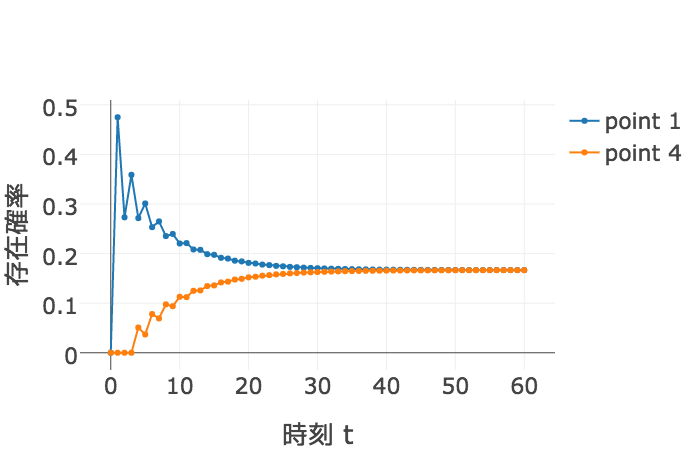
\includegraphics[width=\textwidth]{fig1.png}
  		\caption{時刻 t における地点1,4でのバッタGの存在確率(s=0.05)}
	\end{figure}

	\begin{figure}
  		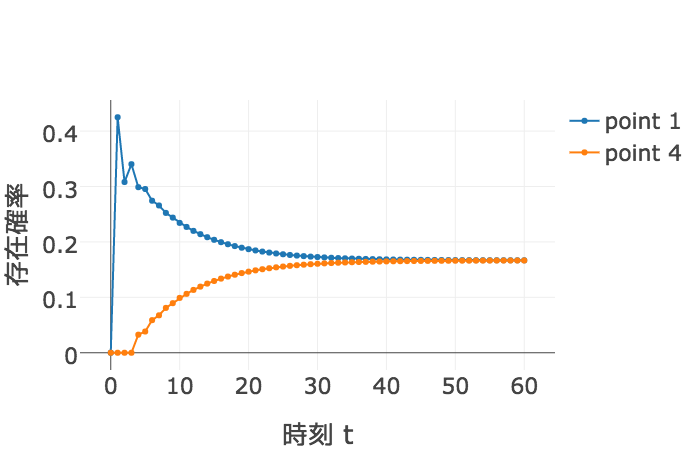
\includegraphics[width=\textwidth]{fig2.png}
  		\caption{時刻 t における地点1,4でのバッタGの存在確率(s=0.15)}
	\end{figure}

	\begin{figure}
  		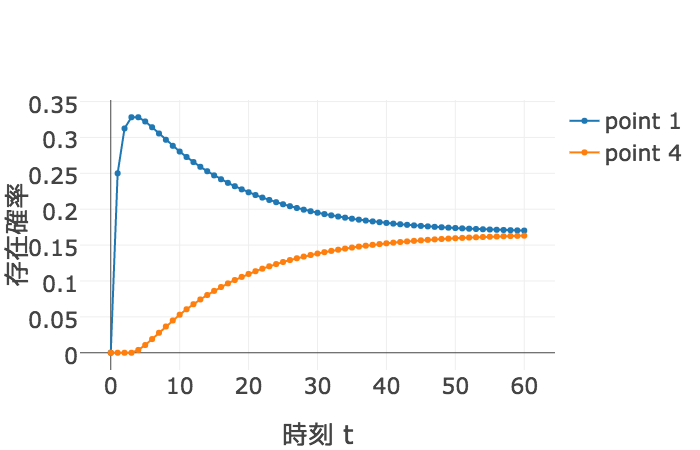
\includegraphics[width=\textwidth]{fig3.png}
  		\caption{時刻 t における地点1,4でのバッタGの存在確率(s=0.5)}
	\end{figure}

	図1,2,3を見ると、sが大きくなるに連れて、オーバーシュートが大きくなり、また、定常値に落ち着くまでの時間が長くなっている事がわかる。

\subsection{パラメータcによるバッタGの振る舞いの変化}
	$t=60$において各地点にGがいる確率をグラフにしたのが、図4,5,6である。

	\begin{figure}
  		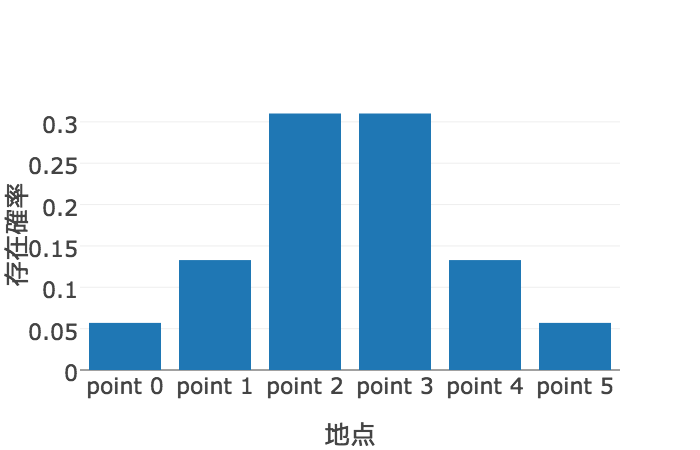
\includegraphics[width=\textwidth]{fig4.png}
  		\caption{ t=60における各地点でのGの存在確率(c=0.7)}
	\end{figure}

	\begin{figure}
  		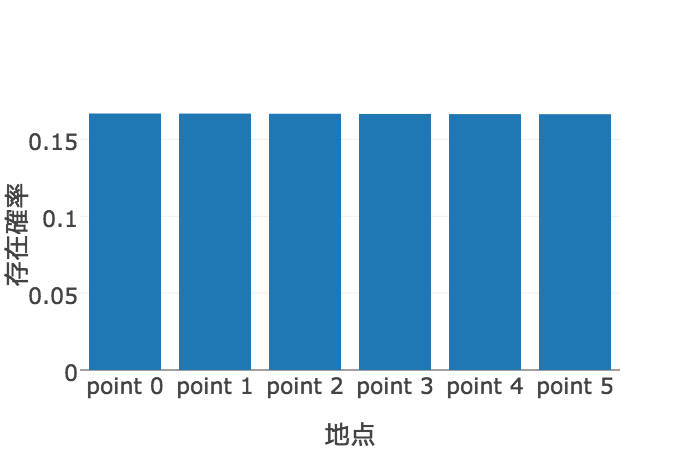
\includegraphics[width=\textwidth]{fig5.png}
  		\caption{ t=60における各地点でのGの存在確率(c=0.5)}
	\end{figure}

	\begin{figure}
  		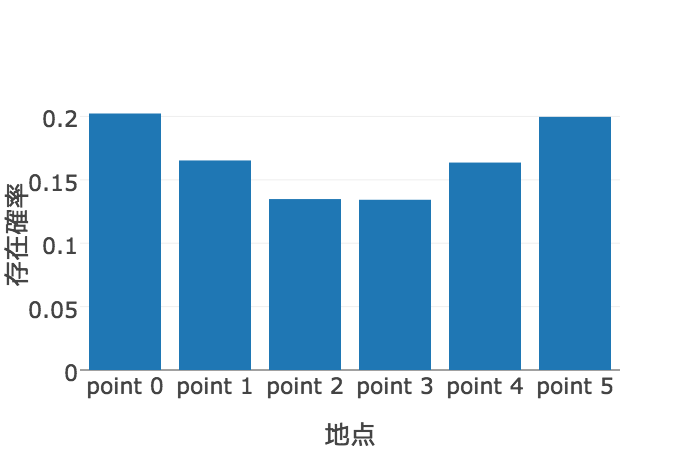
\includegraphics[width=\textwidth]{fig6.png}
  		\caption{ t=60における各地点でのGの存在確率(c=0.45)}
	\end{figure}

	図4,5,6を見ると、cが大きくなるに連れて、中央に近い地点の存在確率が高くなっていることがわかる。
\subsection{ニュートン法による非線形方程式の解}

計算結果として、

\begin{itemize}
	\item (1)に対しては$x = 0.4685126936655117$
	\item (2)に対しては$x = 2.6107790395825665$
\end{itemize}

という解が得られた。


\section{考察}
\subsection{行列とベクトルの演算を行う関数の実装}
	理解しやすいように、またデバッグがしやすいように、抽象度の高い関数を組み合わせて2つの関数を実装したが、科学技術計算において実用レベルのものとしては速度が不安である。
	現実の行列演算ライブラリとして用いられるものを実装するのであれば、C言語で拡張ライブラリを作成する、関数呼び出しを伴わずに実装する、などの工夫が必要となると考えられる。

\subsection{バッタGの移動}
	表1を見ると、sというパラメータは、前の時刻にいた場所に、次の時刻にもいる確率を表していることがわかる。
	その場にとどまる確率(s)が低いほど、tが小さいときにGが地点0から地点1に移動してくる確率が高いため、オーバーシュートが大きくなると考えられる。
	また、その場にとどまる確率(s)が高いほど、ある状態から次の状態に移行する確率が低くなり、変化にはより多くの時間がかかると考えられる。

\subsection{パラメータcによるバッタGの振る舞いの変化}
	表1について、各列の確率を足し合わせると、
	\begin{itemize}
		\item 点0,5に移動してくる確率のそれぞれの合計$P_x = s + 2(1-s)(1-c)$
		\item 点1,4に移動してくる確率のそれぞれの合計$P_y = s + 2(1-s)1 = 1$
		\item 点2,3に移動してくる確率のそれぞれの合計$P_z = s + 2(1-s)c$
	\end{itemize}
	のように表せる。

	これを見るとわかるように、$c = 0.5$のとき、$P_x, P_y, P_z$のどれについても$1$となるので、定常状態においては、どの点にいる確率も等しくなると予想できる。

	また、$c > 0.5$のとき、
		$$P_x < P_y < P_z$$
	となるので、定常状態においては、点0,5にいる確率が一番小さく、点2,3にいる確率が一番大きくなると予想できる。

	同様に、$c < 0.5$のとき、
		$$P_x > P_y > P_z$$
	となることから、それぞれ、定常状態においては、点0,5にいる確率が一番大きく、点2,3にいる確率が一番小さくなると予想できる。

\subsection{ニュートン法による非線形方程式の解}
	以下、便利のため
	\begin{eqnarray*}
       f_1(x) & = & - 2.2 x^4 + 3.5x^3 + 4.1x^2 + 3.3x - 2.7 \\
       f_2(x) & = & - {\rm cos}(2x+2) + {\rm exp}(x+1) - 2x -30
	\end{eqnarray*}
	とおく。

	$f_1$は、$|f_1(x_{k})| < \epsilon$も$|x_{k} - x_{k-1}| < \epsilon$も満たして終了している。
	$f_1$については、$f_1(x)$が$0$になってしまったため、それ以上の修正が行われなくなったと考えられる。

	$f_2$は、$|x_{k} - x_{k-1}| < \epsilon$は満たされているが、$|f_2(x_{k})| < \epsilon$は満たされず、実行回数の上限によって終了している。
	しかし、終了直前については、$x$の値は変化しておらず、float64型の精度の上限いっぱいまで正確な近似解を求めていると考えられる。

	このことから、$|f_2(x_{k})| < \epsilon$が満たされないのは、$f_2$の中には指数関数が入っているため、$x$の小さな変化に対しても、鋭敏に$f_2(x)$の値が変化してしまうことが原因であると考えられる。
	float64型の誤差は10進数でおおよそ$10^{-16}$程度であるので、$|x_{k} - x_{k-1}| < \epsilon$が成立する$x_{k}$の近傍での$f_2$の誤差$\Delta f_2$は、
	\begin{eqnarray*}
		\Delta f_2 & \approx & \frac{\partial f_2}{\partial x} \Delta x \\
				   & \approx & e^{2.6107790395825665+1} \times 10^{-16} \\
				   & \approx & 3.7 \times 10^{-15}
	\end{eqnarray*}
	となり、$10^{-15}$程度は発生することになる。
	実際、$|x_{k} - x_{k-1}| < \epsilon$が満たされたときの$|f(x)|$の値は、$10^{-15}$程度の値であり、$f_2$の誤差程度の値までは小さくなっていることがわかる。

\end{document}